\documentclass[11pt]{formatting-template}

% mathptmx is a Times Roman look-alike (don't use the times package)
% It isn't clear if Times is required. The OGS manual lists several
% "standard fonts" but never says they need to be used.
% \usepackage{mathptmx}

\usepackage[NoDate]{currvita}
\usepackage{array}
\usepackage{tabularx}
\usepackage{booktabs}
\usepackage{ragged2e}
\usepackage{microtype}
\usepackage[breaklinks=true,pdfborder={0 0 0}]{hyperref}
\usepackage{graphicx}
\AtBeginDocument{%
	\settowidth\cvlabelwidth{\cvlabelfont 0000--0000}
}

% OGS recommends increasing the margins slightly.
\increasemargins{.1in}

\usepackage[english]{babel}
\usepackage{blindtext}

\usepackage{url}

\usepackage[super,sort&compress]{natbib}

\overfullrule5pt

%%%%%%%%%%%%%%%%%%%%%%%%%%%%%%%%%%%%%%%%%%%%%%%%%%%%%%%%%%%%%%%%%%%%%%%%%%%%%%%%
% Thesis Title & Author Information
\title{My title here}
\author{Author Name}
\degree{Bioinformatics \& Systems Biology}{Doctor of Philosophy}

% Thesis Committee Members
\chair{Professor One}
\cochair{Professor Two} 
\committee{Professor Three}
\committee{Professor Four} % alphabetical order required
\committee{Professor Five}
\degreeyear{2023}

%%%%%%%%%%%%%%%%%%%%%%%%%%%%%%%%%%%%%%%%%%%%%%%%%%%%%%%%%%%%%%%%%%%%%%%%%%%%%%%%
\begin{document}

% Begin with front matter and so forth
\frontmatter
\maketitle{}
\makecopyright{}
\makesignature{}

%%%%%%%%%%%%%%%%%%%%%%%%%%%%%%%%%%%%%%%%%%%%%%%%%%%%%%%%%%%%%%%%%%%%%%%%%%%%%%%%
% Dedication
%%%%%%%%%%%%%%%%%%%%%%%%%%%%%%%%%%%%%%%%%%%%%%%%%%%%%%%%%%%%%%%%%%%%%%%%%%%%%%%%
\begin{dedication}
	\setsinglespacing{}
	\parindent0pt\parskip\baselineskip{}
	\vskip0pt plus.25fil
	\begin{center}
		
		$\cdots$

		This dissertation is dedicated to \dots\\
		and \textit{Person}.
		
	\end{center}
\end{dedication}

%%%%%%%%%%%%%%%%%%%%%%%%%%%%%%%%%%%%%%%%%%%%%%%%%%%%%%%%%%%%%%%%%%%%%%%%%%%%%%%%
% Epigraph
%%%%%%%%%%%%%%%%%%%%%%%%%%%%%%%%%%%%%%%%%%%%%%%%%%%%%%%%%%%%%%%%%%%%%%%%%%%%%%%%
\begin{epigraph}
	\vskip0pt plus.5fil
	\vfil\vfil
	\setsinglespacing{}
	{ \flushright{
		This is an epigraph\\
		about epigraphs.\\
		}
		\vskip\baselineskip{}
		- \textit{Author Name}\par
	}
	\vfil\vfil\vfil
\end{epigraph}

%%%%%%%%%%%%%%%%%%%%%%%%%%%%%%%%%%%%%%%%%%%%%%%%%%%%%%%%%%%%%%%%%%%%%%%%%%%%%%%%
% Table of Contents, Figures, Tables, Etc.
%%%%%%%%%%%%%%%%%%%%%%%%%%%%%%%%%%%%%%%%%%%%%%%%%%%%%%%%%%%%%%%%%%%%%%%%%%%%%%%%
% Next comes the table of contents, list of figures, list of tables,
% etc. If you have code listings, you can use \listoflistings (or
% \lstlistoflistings) to have it be produced here as well. Same with
% \listofalgorithms.

\tableofcontents
\listoffigures
\listoftables

%%%%%%%%%%%%%%%%%%%%%%%%%%%%%%%%%%%%%%%%%%%%%%%%%%%%%%%%%%%%%%%%%%%%%%%%%%%%%%%%
% Acknowledgements
%%%%%%%%%%%%%%%%%%%%%%%%%%%%%%%%%%%%%%%%%%%%%%%%%%%%%%%%%%%%%%%%%%%%%%%%%%%%%%%%
\begin{acknowledgements}
	I would like to thank the following people for their support throughout my graduate school journey. \textit{Professor One} for being a great advisor. \textit{Professor Two} for being a great co-advisor. \textit{Professor Three} for being a great committee member. \textit{Professor Four} for being a great committee member. \textit{Professor Five} for being a great committee member. \textit{Professor Six} for being a great committee member. \textit{Professor Seven} for being a great committee member. \textit{Professor Eight} for being a great committee member. \textit{Professor Nine} for being a great committee member. \textit{Professor Ten} for being a great committee member. \textit{Professor Eleven} for being a great committee member. \textit{Professor Twelve} for being a great committee member. \textit{Professor Thirteen} for being a great committee member. \textit{Professor Fourteen} for being a great committee member. \textit{Professor Fifteen} for being a great committee member. \textit{Professor Sixteen} for being a great committee member. \textit{Professor Seventeen} for being a great committee member. \textit{Professor Eighteen} for being a great committee member. \textit{Professor Nineteen} for being a great committee member. \textit{Professor Twenty} for being a great committee member. \textit{Professor Twenty-One} for being a great committee member. \textit{Professor Twenty-Two} for being a great committee member. \textit{Professor Twenty-Three} for being a great committee member. \textit{Professor Twenty-Four} for being a great committee member. \textit{Professor Twenty-Five} for being a great committee member. \textit{Professor Twenty-Six} for being a great committee member. \textit{Professor Twenty-Seven} for being a great committee member. \textit{Professor Twenty-Eight} for being a great committee member. \textit{Professor Twenty-Nine} for being a great committee member. \textit{Professor Thirty} for being a great committee member. \textit{Professor Thirty-One} for being a great committee member. \textit{Professor Thirty-Two} for being a great committee member. \textit{Professor Thirty-Three} for being a great committee member.
\end{acknowledgements}

%%%%%%%%%%%%%%%%%%%%%%%%%%%%%%%%%%%%%%%%%%%%%%%%%%%%%%%%%%%%%%%%%%%%%%%%%%%%%%%%
% Vita
%%%%%%%%%%%%%%%%%%%%%%%%%%%%%%%%%%%%%%%%%%%%%%%%%%%%%%%%%%%%%%%%%%%%%%%%%%%%%%%%
\begin{vita}
\noindent
\begin{cv}{}
\begin{cvlist}{}
	\item[2012] High School Diploma\\
		University City High School
	\item[2012--2016] B.S. in Usefulology\\
		University of California, San Diego
	\item[2016--2023] Ph.D. in Bioinformatics \& Systems Biology\\
		University of California, San Diego
\end{cvlist}
\end{cv}

%%%%% PUBLICATIONS %%%%%
\publications{}

\noindent \textit{Author names marked with $\dagger$ indicate shared first co-authorship.} \newline
\noindent \textit{Publications marked with $\triangle$ are included in this text.} \newline

\noindent \textbf{Author Name} and Professor One. ``My first publication.'' \textit{Journal of Publications}, 2020. $\triangle$ \newline

%%%%% FIELDS OF STUDY %%%%% 
% This section was omitted within this thesis as it was optional.

\end{vita}

%%%%%%%%%%%%%%%%%%%%%%%%%%%%%%%%%%%%%%%%%%%%%%%%%%%%%%%%%%%%%%%%%%%%%%%%%%%%%%%%
% Dissertation Abstract 
%%%%%%%%%%%%%%%%%%%%%%%%%%%%%%%%%%%%%%%%%%%%%%%%%%%%%%%%%%%%%%%%%%%%%%%%%%%%%%%%
\begin{dissertationabstract}
	An abstract should provide a clear impression of the content and major divisions of the dissertation or thesis. Abstracts of doctoral dissertations must not exceed 350 words. 
\end{dissertationabstract}

%%%%%%%%%%%%%%%%%%%%%%%%%%%%%%%%%%%%%%%%%%%%%%%%%%%%%%%%%%%%%%%%%%%%%%%%%%%%%%%%
% Main Text of the Dissertation
%%%%%%%%%%%%%%%%%%%%%%%%%%%%%%%%%%%%%%%%%%%%%%%%%%%%%%%%%%%%%%%%%%%%%%%%%%%%%%%%
\mainmatter{}

\begin{dissertationintroduction}
    
\setcounter{chapter}{0}
\chapter*{Introduction}

\label{chap:introduction}

\section{The importance of RNA localization}
The fundamental unit of life is the cell, from unicellular organisms like bacteria to complex multicellular organisms like humans. While it is convenient to think of cells as amorphous liquid bags of lipids, proteins and sugars, cells are highly structured and and regulated. The genome serves as the template for RNAs; they are synthesized then modified by tightly orchestrated processes such as splicing, localization, translation, and degradation so a cell can function. We can measure the abundance of a cell's transcriptome, the complete repertoire of RNA, to loosely quantify cellular activity. But what do these molecules physically interact with? Where do these interactions occur in the cell and what causes them to interact? This layer of regulation, RNA localization, plays an important role in cell processes such as protein synthesis, signaling pathways and RNA degradation. For example, mRNAs exhibit asymmetric distributions in developing \textit{Drosophila melanogaster} embryos, compartment-specific localization in the neurites of neurons, and colocalization with the actin cytoskeleton in fibroblasts \cite{buxbaumRightPlaceRight2015}. The prevalence of RNA localization across diverse cell types and organisms indicate that it is a highly conserved process. Abnormal RNA localization has also been associated with many neurodegenerative diseases such as Huntington's disease (HD), where defects in axonal mRNA transport and subsequent translation in human spiny neurons lead to cell death and neurodegeneration \cite{fernandopulleRNATransportLocal2021}. Despite these repeated observations, the determinants of localization are not well understood.

\section{Spatial transcriptomics technology}

While we can easily quantify RNA expression with sequencing, RNA imaging techniques have traditionally been limited to visualizing a handful of species per experiment. However, recent multiplexed imaging technologies have unlocked much higher experimental throughput at hundreds to thousands of species, enabling nearly transcriptome-scale analysis of spatial RNA distributions. Single-molecule fluorescent in situ hybridization\cite{rajImagingIndividualMRNA2008} (smFISH) was one of the first popularized techniques able to image RNAs by species using synthesized complementary DNA (cDNA) sequences with fluorochromes. The cDNA probes hybridize to RNA targets and emit light upon excitation, which is captured by microscope cameras as dots of light, less than a micron wide. By designing specific probes for each RNA species of interest, it is possible to image multiple unique species at a time in the same cells. In order to scale to target hundreds to tens of thousands of unique RNA species, recent combinatorial FISH techniques compress the number of imaging rounds needed to identify each target by designing sets of barcodes that fluoresce in a specific sequence of images for individual RNA species. For example, MERFISH\cite{chenSpatiallyResolvedHighly2015} is one technique using a barcoding scheme that allows detection of 10,000 unique RNA targets in 69 rounds of sequential images. At such a scale, we can begin to study the RNA life cycle from a new perspective, by observing the spatial organization of the transcriptome and uncovering principles of RNA regulation linked to localization. The set of technologies able to capture the spatial organization of RNA in cells and tissue is termed spatial transcriptomics.\footnote{In addition to imaging-based methods, there exists a host of slide-based methods that are just as prevalent but not in the scope of this work. In summary these methods use a grid of barcoded wells on slides to capture and sequence transcripts. The location of each well is used to spatially map transcripts.}

\section{Current analysis trends}

As spatial transcriptomics assays reaches the scientific main stream \cite{marxMethodYearSpatially2021}, there is a growing need for scalable analysis software and computational infrastructure. The most robust and enduring tools adhere to FAIR principles\cite{wilkinsonFAIRGuidingPrinciples2016} — Findability, Accessibility, Interoperability, and Reusability—a set of standards proposed by researchers to maximize reuse of research objects for advancing scientific discovery. Data management strategies such as version control, software containerization, and pipeline management are often second priority in academic research. Consequentially, many academic tools do not see use outside of their initial projects and collaborations due to low adoption. Mainstream media attention around the “reproducibility crisis” and high profile cases of academic fraud have demonstrated the clear value of enforcing FAIR principles for academic research, both to researchers and for building trust with the average citizen. 

The field of spatial transcriptomics has witnessed an evolution of various tools and platforms, each specializing in different aspects of analysis and data handling. For image processing, tools like \textit{multi-fish}\cite{wangEASIFISHThickTissue2021}, \textit{mcmicro}\cite{schapiroMCMICROScalableModular2022}, and \textit{MERlin}\cite{ZhuangLabMERlinMERlin} are tailored specifically for certain technologies. In contrast, \textit{starfish/PIPEFISH}\cite{othersStarfishOpenSource,cisarUnifiedPipelineFISH2023} and \textit{spotfish} (described in this work) attempt to be platform agnostic and focus on pipeline building infrastructure instead of task-specific algorithms. In terms of data structures, \textit{AnnData}\cite{virshupAnndataAnnotatedData2021} specifically supports single-cell data matrices, while \textit{SpatialData}\cite{marconatoSpatialDataOpenUniversal2023}, \textit{SpatialExperiment}\cite{righelliSpatialExperimentInfrastructureSpatiallyresolved2022} offer more complex representations, attempting supporting a spectrum of data modalities and the relationships between them. Single-cell analysis is the \textit{de facto} approach to analyze spatial transcriptomics, and tools such as \textit{Giotto}\cite{driesGiottoToolboxIntegrative2021}, \textit{Squidpy}\cite{pallaSquidpyScalableFramework2021}, \textit{Stereopy}\cite{STOmicsStereopy2023}, \textit{stLearn}\cite{phamStLearnIntegratingSpatial2020}, and \textit{Voyager}\cite{mosesVoyagerExploratorySinglecell2023} are equipped to handle cell-centric functional analyses. Subcellular analysis, which delves deeper into spatial interactions at the molecular level, features tools like \textit{INSTANT}\cite{kumarIntracellularSpatialTranscriptomic2023}, \textit{SpaGNN}\cite{fangSubcellularSpatiallyResolved}, and \textit{FISHfactor}\cite{walterFISHFactorProbabilisticFactor}. \textit{Bigfish}\cite{imbertFISHquantV2Scalable2022} and \textit{Bento}\cite{mahBentoToolkitSubcellular2022} in this category are examples of software packages developed with FAIR principles in mind. Overall, this brief listing highlights the growing interest in the budding field of spatial transcriptomics and the need for FAIR tools to support the maturation of the field.


\setlength\LTleft{0pt}
\setlength\LTright{0pt}
\begin{small}
    \renewcommand\thetable{0.1}
    \begin{landscape} % this table is long
        \begin{longtable}{l l l l l l l}
            % Define the table title in the table of contents
            \caption{Assessment of FAIR principles in spatial transcriptomics tools}\label{tab:spatial-tx tools assessment}
            \\ \hline 

            % Define the table columns for the first and all subsequent pages
            \multicolumn{1}{l}{\textbf{Category}} & \multicolumn{1}{l}{\textbf{Tool}} & \multicolumn{1}{l}{\textbf{Spatial-Tx Compatible}} & \multicolumn{1}{l}{\textbf{Findability}} & \multicolumn{1}{l}{\textbf{Accessibility}} & \multicolumn{1}{l}{\textbf{Interoperability}} & \multicolumn{1}{l}{\textbf{Reusability}} \\ \hline \endhead 

            % \multicolumn{7}{l}%
            % {{\textbf{\tablename\ \theHtable{}.} Assessment of FAIR principles in spatial transcriptomics tools, \textit{continued from previous page}}} \\
            % \hline 
            
            % Define the table footer for the first and all subsequent pages
            \hline \multicolumn{7}{r}{\textit{Continued on next page}} \\ \hline \endfoot
            \hline \endlastfoot
            
            % Start table content

            %%%%% %%%%% %%%%% %%%%% %%%%% %%%%% %%%%% %%%%% %%%%% %%%%% %%%%% %%%%%
            \textbf{Image Processing} & easi-fish & ~ & x & x & x & x \\ 
            \textbf{} & MERlin & MERFISH only & x & x & x & x \\ 
            \textbf{} & mcmicro & ~ & x & x & x & x \\ 
            \textbf{} & starfish/PIPEFISH & x & x & ~ & ~ & x \\ 
            \textbf{} & spotfish & x & x & x & x & x \\ 
            \textbf{Data Structure} & AnnData & ~ & x & x & x & x \\ 
            \textbf{} & SpatialData & x & x & x & x & x \\ 
            \textbf{} & SpatialExperiment & x & x & x & x & x \\ 
            \textbf{Single-Cell Analysis} & Giotto & x & x & x & x & x \\ 
            \textbf{} & Squidpy & x & x & x & x & x \\ 
            \textbf{} & Stereopy & x & x & x & x & x \\ 
            \textbf{} & stLearn & x & x & x & x & x \\ 
            \textbf{} & Voyager & x & x & x & x & x \\ 
            \textbf{Subcellular Analysis} & INSTANT & x & ~ & ~ & ~ & ~ \\ 
            \textbf{} & SpaGNN & x & ~ & ~ & ~ & ~ \\ 
            \textbf{} & FISHfactor & x & ~ & ~ & ~ & x \\ 
            \textbf{} & Bigfish & ~ & x & x & ~ & x \\ 
            \textbf{} & Bento & x & x & x & x & x \\ 
        \end{longtable}
    \end{landscape}
\end{small}


\end{dissertationintroduction}

\chapter{Bento: A toolkit for subcellular analysis of spatial transcriptomics data}
\label{chap:chapter 1}

%%%%%%%%%%%%%%%%%%%%%%%%%%%%%%%%%%%%%%%%%%%%%%%%%%%%%%%%%%%%%%%%%%%%%%%%%%%%%%%%
\section{Introduction}
%%%%%%%%%%%%%%%%%%%%%%%%%%%%%%%%%%%%%%%%%%%%%%%%%%%%%%%%%%%%%%%%%%%%%%%%%%%%%%%%

The spatial organization of molecules in a cell is essential for performing their functions. While protein localization\cite{thulSubcellularMapHuman2017} and disease-associated mislocalization are well appreciated\cite{laurilaPredictionDiseaserelatedMutations2009,parkProteinLocalizationPrincipal2011}, the same principles for RNA have begun to emerge. For instance, the spatial and temporal regulation of RNA play a crucial role in localized cellular processes such as cell migration and cell division\cite{lecuyerGlobalAnalysisMRNA2007,bovairdBiologicalFunctionsRegulatory2018}, as well as specialized cell functionalities like synaptic plasticity\cite{dasTravelsMRNAsNeurons2019,sahooAxonalMRNATransport2018,kugelgenConservationCoreNeurite2020}. Mislocalization of RNA has been associated with diseases such as Huntington's disease (HD), where defects in axonal mRNA transport and subsequent translation in human spiny neurons lead to cell death and neurodegeneration\cite{culverHuntingtonDiseaseProtein2016,romoFreshLookHuntingtin2018,whiteHuntingtinDifferentiallyRegulates2015,fernandopulleRNATransportLocal2021}.

The study of subcellular RNA localization necessitates single-molecule measurements. Since the development of single-molecule fluorescent in situ hybridization (smFISH), recent advances in multiplexed methods such as MERFISH\cite{chenRNAImagingSpatially2015}, seqFISH+\cite{engTranscriptomescaleSuperresolvedImaging2019}, HybISS\cite{gyllborgHybridizationbasedSituSequencing2020}, and Ex-Seq\cite{alonExpansionSequencingSpatially} have enabled RNA localization measurements at near transcriptome scales, while maintaining single-molecule resolution. A number of computational toolkits, such as Squidpy\cite{pallaSquidpyScalableFramework2021}, stLearn\cite{phamStLearnIntegratingSpatial2020}, Giotto\cite{driesGiottoToolboxIntegrative2021}, Seurat\cite{butlerIntegratedAnalysisSingle2017}, and Scanpy\cite{wolfSCANPYLargescaleSinglecell2018} enabled the characterization of tissue architecture, cell-cell interactions, and spatial expression patterns. Despite the single-molecule measurements in spatial transcriptomics, these analytical approaches are limited to investigating spatial variation at the multicellular scale and lack the ability to investigate subcellular organization. To further our understanding of RNA localization and its function in normal and abnormal cell activity, we need to expand our analytical capacity to the subcellular scale.

Recent methods such as FISH-quant-v2\cite{imbertFISHquantV2Scalable2022} and FISHFactor\cite{walterFISHFactorProbabilisticFactor} identify subcellular patterns describing the spatial distribution of RNA species, but are unable to annotate more than a single gene per cell or are limited to analyze at most 20,000 molecules on accessible computing resources. In contrast, a single spatial transcriptomics experiment measures at least hundreds to thousands of genes across hundreds of thousands of cells. Additionally, methods such as ClusterMap\cite{heClusterMapMultiscaleClustering2021} and Baysor\cite{petukhovBayesianSegmentationSpatially2020} highlight the potential for transcript locations alone to inform meaningful domains such as cell and nuclear regions Using spatial proteomics data, CAMPA\cite{spitzerLearningConsistentSubcellular} and Pixie\cite{liuRobustPhenotypingHighly2023} utilize subcellular spatial variation in protein abundance to identify subcellular regions and annotate pixel-level features. 

Building on these promising approaches, we present Bento, an open-source Python toolkit for scalable analysis of spatial transcriptomics data at the subcellular resolution. Bento ingests single-molecule resolution data and segmentation masks, utilizing geospatial tools (GeoPandas\cite{GeopandasGeopandasV0}, Rasterio\cite{gilliesRasterioGeospatialRaster}) for spatial analysis of molecular imaging data, and data science tools including SciPy\cite{virtanenSciPyFundamentalAlgorithms2020}, and Tensorly\cite{kossaifiTensorLyTensorLearning2019} for scalable analysis of high-dimensional feature matrices. Furthermore, Bento is a member of the Scverse ecosystem, enabling integration with Scanpy\cite{wolfSCANPYLargescaleSinglecell2018}, Squidpy\cite{pallaSquidpyScalableFramework2021}, and more than thirty other single-cell omics analysis tools.

%%%%%%%%%%%%%%%%%%%%%%%%%%%%%%%%%%%%%%%%%%%%%%%%%%%%%%%%%%%%%%%%%%%%%%%%%%%%%%%%
\section{Results}
%%%%%%%%%%%%%%%%%%%%%%%%%%%%%%%%%%%%%%%%%%%%%%%%%%%%%%%%%%%%%%%%%%%%%%%%%%%%%%%%

\subsection{Overview of Bento data infrastructure for subcellular analysis}

In order to facilitate a flexible workflow, Bento is generally compatible with molecule-level resolution spatial transcriptomics data (Fig. 1A), such as datasets produced by MERFISH\cite{chenSpatiallyResolvedHighly2015}, seqFISH+\cite{engTranscriptomescaleSuperresolvedImaging2019}, CosMx (NanoString)\cite{heHighplexMultiomicAnalysis2021}, Xenium (10x Genomics)\cite{janesickHighResolutionMapping2022,leeFluorescentSituSequencing2015}, and Molecular Cartography (Resolve Biosciences)\cite{huDynamicControlMetabolic}. Bento's workflow takes as input 1. 2D spatial coordinates of transcripts annotated by gene, and 2. segmentation boundaries (e.g. cell membrane, nuclear membrane, and any other regions of interest) (Fig. 1B). While 3D molecular coordinates are commonly included, 3D segmentation information is limited to z-stacked 2D segmentation, limiting its usability. If available, Bento can also handle arbitrary sets of segmentations for other subcellular structures or regions of interest. These inputs are stored in the AnnData data format\cite{virshupAnndataAnnotatedData2021}, which links cell and gene metadata to standard count matrices, providing compatibility with standard single-cell RNA-seq quality control and analysis tools in the Scverse ecosystem\cite{wolfSCANPYLargescaleSinglecell2018}. With a data structure for segmentation boundaries and transcript coordinates in place, Bento can easily compute spatial statistics and measure spatial phenotypes to build flexible multidimensional feature sets for exploratory subcellular analysis and utilize these spatial metrics to augment quality control (Fig. 1C).

\begin{figure}[h]
    \centering
    \includegraphics[width=\textwidth]{1_figures-and-files/Fig1.pdf}
    \caption[Workflow and functionality of the Bento toolkit.]{\textbf{Workflow and functionality of the Bento toolkit.} A. Single-molecule resolved spatial transcriptomics data from commercial or custom platforms are ingested into Bento where it is converted to the AnnData format (B.), where it can be manipulated with Bento as well as a wide ecosystem of single-cell omics tools. C. Geometric statistics are illustrated for the seqFISH+ dataset, including metrics describing cell and nuclear geometries and cell density to assess overall data quality. D. Bento has a standard interface to perform a wide variety of subcellular analyses.}
    \label{fig:1 bento overview}
\end{figure}

Bento offers a precise yet flexible palette of novel complementary subcellular analyses (Fig. 1D). We present RNAforest, a multilabel approach for annotating RNA localization patterns adapted from FISH-quant v2\cite{imbertFISHquantV2Scalable}. We find that many RNAs are spatially distributed according to gene function. We then implement RNAcoloc, a context-specific approach to quantify colocalization to characterize how genes colocalize with each other in a compartment-specific manner. Having established systematic patterning and organization of RNA transcripts, we demonstrate RNAflux, an unsupervised method for semantic segmentation of subcellular domains. RNAflux first quantifies subcellular expression gradients at pixel resolution before identifying consistent subcellular domains via unsupervised clustering. We demonstrate the utility of Bento's tools characterizing subcellular organization in two spatial transcriptomics datasets, a 10k gene MERFISH dataset of U2-OS cells and a 130 gene seqFISH+ dataset of 3T3 cells. We find that RNA localization patterns are associated with known gene function, and that genes with similar localization patterns are functionally related. We also find that genes with similar localization patterns are co-regulated at the transcriptional level. Finally, we find that RNAflux identifies subcellular domains that are consistent across cells and are associated with known subcellular structures.



\subsection{RNAforest: Utilizing subcellular landmarks to predict RNA subcellular localization}

In computer vision, key points or landmarks are commonly used for tasks like facial recognition\cite{violaRapidObjectDetection2001} and object detection. Analogous to these classical applications, we derive spatial features using cell and nucleus boundaries as landmarks to predict RNA localization patterns from spatial summary statistics. Building on the summary statistics used for classifying smFISH data in FISH-quant v2\cite{imbertFISHquantV2Scalable2022}, RNAforest consists of an ensemble of five binary random forest classifiers rather than a single multi-classifier model to assign one or more labels. These pattern labels, adapted from several high-throughput smFISH imaging experiments in HeLa cells\cite{battichImagebasedTranscriptomicsThousands2013,stoegerComputerVisionImagebased2015,samacoitsComputationalFrameworkStudy2018,chouaibDualProteinmRNALocalization2020}, are broadly applicable to eukaryotic cells: (i) nuclear (contained in the volume of the nucleus), (ii) cytoplasmic (diffuse throughout the cytoplasm), (iii) nuclear edge (near the inner/outer nuclear membrane), (iv) cell edge (near the cell membrane), and (v) none (complete spatial randomness). It is important to note, as was done previously in  FISH-quant v2\cite{imbertFISHquantV2Scalable2022} that because of the 2D nature of the dataset, RNA that is in truth cytoplasmic but above or below the nucleus will still appear as though in the nucleus when collapsed in the z-dimension. As we use the FISH-quant v2 pattern simulation framework, this is accounted for in the training dataset.

We used the FISH-quant v2 simulation framework to generate realistic ground-truth data\cite{samacoitsComputationalFrameworkStudy2018}. Each sample is defined as a set of points with coordinates in two dimensions, representing the set of observed transcripts for a gene in a particular cell. In total, we simulated 2,000 samples per class for a total of 10,000 samples (Methods). We used 80\% of the simulated data for training and held out the remaining 20\% for testing. Each sample is encoded by a set of 13 input features, describing characteristics of its spatial point distribution, including proximity to cellular compartments and extensions (features 1-3), measures of symmetry about a center of mass (features 4-6), and measures of dispersion and point density (feature 7-13) (Fig. 2A). These features are normalized to morphological properties of the cell to control for variability in cell shape. A detailed description of every feature is described in Supp. Table 1. 

\begin{figure}[p]
    \centering
    \includegraphics[width=\textwidth]{1_figures-and-files/Fig2.pdf}
    \caption[Subcellular localization pattern identification with RNAforest.]{\textbf{Subcellular localization pattern identification with RNAforest.} A. Thirteen spatial summary statistics are computed for every gene-cell pair describing the spatial arrangement of molecules and boundaries in relation to one another. The features are inputs for RNAforest, a multilabel ensemble classifier which assigns one or more subcellular localization labels: cell edge, cytoplasmic, nuclear, nuclear edge, and none. Top 10 genes for each label visualized for each label other than “none” in B. U2-OS cells, and C. 3T3 cells. D. and E. show the proportion of measured transcripts assigned to each label. F. and G. show the relative label proportion across cells for each gene and is colored by the majority label (F and G). H. Top 5 consistent genes for each label. I. ssGEA identifies enrichment of GO cellular component domains for each label in the 3T3 cell dataset.
    }
    \label{fig:2 RNAforest localization pattern identification}
\end{figure}

We applied RNAforest on the MERFISH dataset measuring 130 genes (low plexity) in U2-OS cells and high detection efficiency per gene (111 molecules per gene per cell on average), and on the seqFISH+ dataset measuring 10,000 genes (very high plexity) but lower detection efficiency (8 molecules per gene per cell on average) (Fig. 2B-C, Supp. Fig. 1). In agreement with previous work characterizing RNA localization of 411 genes\cite{chouaibDualProteinmRNALocalization2020}, we find that genes commonly exhibit variability in localization across cells. This suggests that heterogeneity in localization likely generalizes to the entire transcriptome. Of the localization patterns besides ``none'', ``nuclear'' was the most common (22.1\%) in the U2-OS osteosarcoma cells (Fig. 2D \& 2F), while ``cell edge'' was the most common (15.9\%) in the 3T3 fibroblast cells (Fig. 2E \& 2G). 

In the U2-OS cells, we found many genes to have preferential localization in different subcellular compartments (Fig. 2H). In agreement with our RNAflux findings, we find genes known to localize to the nucleus\cite{moffittHighthroughputSinglecellGeneexpression2016,kumarIntracellularSpatialTranscriptomic2023} to be frequently labeled ``nucleus'' (MALAT1, SOD2) and genes encoding secreted extracellular proteins\cite{chenRNAImagingSpatially2015} to be frequently labeled ``nuclear edge'' (FBN1, FBN2). As expected, we find genes preferentially ``nuclear'' and ``nuclear edge'' localized to mirror nucleus and endoplasmic reticulum genes found in a 10k genes MERFISH study of U2-OS cells that included ER staining\cite{xiaSpatialTranscriptomeProfiling2019} (Supp. Fig. 2, Methods). Leveraging the 3T3 seqFISH+ dataset's higher plexity, we were able to ask whether genes with similar localization preference are functionally related. We applied gene set enrichment analysis to gene localization frequencies to identify enriched gene ontology terms\cite{thegeneontologyconsortiumGeneOntologyResource2021} (Fig. 2I, Methods). Secretory processes were enriched in the nucleus and nuclear edge, which may be linked to increased transcription of fibroblast-related functions. Cell edge enriched pathways consisted of those with the cell membrane as their site of function (e.g. endocytosis and tight junction suggesting local translation of these genes). Additionally, the term for cell cycle was significantly enriched in the cytoplasm only. Genes without strong localization preference (most frequently ``none'') were not significantly associated with any pathways. These genes likely do not undergo active transport and are functionally independent of local translation. 
RNAforest gives a user a facile method for annotating RNA localization patterns and quantifying heterogeneity in a transcriptome-wide manner independent of RNA abundance. Beyond known RNA localizations, we find that transcript location is generally associated with known gene function, alluding to the systematic spatial regulation of RNA transport. We foresee RNAforest will be a valuable addition to characterize RNA localization across diverse spatial transcriptomics datasets. 

\subsection{RNAcoloc: An approach for context-specific RNA colocalization}

In geospatial information processing, a fundamental feature that is often gleaned from large datasets is the colocation of objects (e.g. gleaning socialization metrics from cell phone colocation data in Singapore\cite{xuHowFriendsShare2017}). Colocation is similarly valuable in understanding co-translation and interaction networks of genes in a biological context\cite{zengSpatiallyResolvedSinglecell2023}. Recent spatial transcriptomics approaches have used a number of colocalization metrics from the geographic information systems and ecology fields e.g. the bivariate versions of the Ripley's K function (also known as cross-k-function)\cite{ripleySecondorderAnalysisStationary1976}, Moran's I\cite{tiefelsdorfModellingSpatialProcesses2006}, and the join count statistic\cite{cliffSpatialProcessesModels1981}. These metrics are designed to measure spatial associations between two populations i.e. gene A transcripts and gene B transcripts. However, it is more appropriate to think of all transcripts in a single cell from a single population; after all, RNA transcription and localization is not completely stochastic. We have shown that the subcellular distribution of RNA is highly structured with RNAforest. As such, we developed RNAcoloc, an approach that combines  the Colocation Quotient (CLQ)\cite{leslieColocationQuotientNew2011} metric and tensor decomposition for context-specific RNA colocalization (Methods). The CLQ is a colocalization statistic that is capable of accounting for the biophysical properties of RNA spatial distributions. First, the CLQ considers how clustered the overall RNA population is in a cell and measures whether specific pairs of genes are more clustered than expected given the spatial pattern of the overall population. Second, the CLQ is inherently asymmetric, and captures the direction of attraction i.e. the attraction of gene A to gene B is not the same as the attraction of gene B to gene A. This is most common when gene A and gene B have very different expression levels, which is prevalent due to overdispersion in gene expression data.

RNAcoloc calculates CLQ scores for each gene per cell in a compartment-specific manner, such that each sample has 2 scores, a nucleus and cytoplasm CLQ score. An initial comparison of global colocalization between nuclear and cytoplasmic fractions unsurprisingly found that transcripts from the same gene tend to cluster more tightly with themselves than with transcripts from other genes (Fig. 3B). Additionally, self-colocalization is significantly stronger in the cytoplasm than in the nucleus. In conjunction with our findings from RNAforest analysis that genes of the same localization pattern tend to have similar functions, this suggests that the RNAs are more tightly spatially regulated once exported from the nucleus. 

By calculating CLQ scores for every gene-gene pair across compartments, RNAcoloc constructs a tensor of shape P x C x S where P, C, and S represent the number of gene-gene pairs, cells, and compartments, respectively (Fig. 3A, Methods). 

RNAcoloc then applies tensor decomposition — specifically, non-negative parallel factor analysis — a data-driven, unsupervised approach for discovering substructure in high-dimensional data\cite{kossaifiTensorLyTensorLearning2019,shashuaNonnegativeTensorFactorization2005} to decompose the U2-OS dataset colocalization tensor into k = 4 ``colocalization factors''. The number of factors was determined using the elbow method heuristic, optimizing for the root mean squared error (RMSE) reconstruction loss (Methods). Unlike matrix dimensionality reduction methods, such as PCA, the order of the components (factors) is unassociated with the amount of variance explained. Each of the 4 colocalization factors is composed of 3 loading vectors, which correspond to the compartments, cells and gene pairs. Higher values denote a stronger association with that factor. Crucially for interpretation, factors derived from tensor decomposition are not mutually exclusive and share overlapping sets of associated compartments, cells, and gene pairs.

\begin{figure}[p]
    \centering
    \includegraphics[width=\textwidth]{1_figures-and-files/Fig3.pdf}
    \caption[Compartment-specific RNA colocalization with RNAcoloc.]{\textbf{Compartment-specific RNA colocalization with RNAcoloc.} A. Transcripts are separated by compartment (nucleus and cytoplasm) before CLQ scores are calculated for every gene pair across all cells. This yields a cell x gene pair x compartment tensor. B. Comparison of log CLQ distributions for gene pairs and self-pairs, further categorized by compartment. C. Tensor decomposition yields 4 factors. From left to right, the three heatmaps show the loadings of each factor for each dimension – compartments, cells, and gene pairs. Only the top 5 associated gene pairs for each factor are shown. D. Top examples of compartment-specific colocalized gene pairs. Black scale bars denote 10 um.
    }
    \label{fig:3 RNAcoloc colocalization analysis}
\end{figure}

These trends are broken down into unique combinations of colocalization behavior (Fig. 3C). Factor 0 captures gene pairs in a subpopulation of cells that tend to colocalize across the entire cell, with pairs including SLC38A1 showing the strongest signal. Factor 3 describes gene pairs in mostly the same cell subpopulation, that colocalize specifically in the cytoplasm. Pairs including PIK3CA dominate this behavior. Interestingly, PIK3CA and DYNC1H1 transcripts colocalize cytoplasmically. While little is known about their RNA interactions, PIK3CA and other members of the PI3K pathway are known regulators of mitotic organization, including the regulation of dynein and dynactin motor proteins. DYNC1H1 specifically encodes cytoplasmic dynein, a motor protein critical for spindle formation and chromosomal segregation in mitosis\cite{gassmannDyneinKinetochore2023}. In the complementary cell population, Factors 1 and 2 highlight colocalized gene pairs in the nucleus and cytoplasm respectively. Notably, Factor 2 associated cells have high loadings for MALAT1 and CNR2 in the cytoplasm and low loadings in the nucleus. Even though MALAT1 is abundantly localized to the nucleus, this demonstrates that the CLQ score identifies gene pairs colocalizing more than expected given the overabundance of MALAT1 relative to CNR2, whereas other approaches seem confounded by large differences in expression\cite{kumarIntracellularSpatialTranscriptomic2023}.

We demonstrate the ability of RNAcoloc to quantify compartment-specific gene-pair colocation by exploring cytoplasmic vs. nuclear colocalization. As we found separately with RNAforest, RNAcoloc analysis finds evidence that RNA transport is spatially regulated, especially after nuclear export. We highlight several examples of colocalization suggesting how RNA localization allows the same gene to have multiple functions in a spatially-dependent fashion i.e. depending on its molecular neighbors and local environment\cite{guptaMoonlightingEnzymesWhen2023,gnannIlluminatingNongeneticCellular2021}. We foresee RNAcoloc will be increasingly relevant as many spatial technologies are beginning to image proteins along with RNA, which can be used to delineate more granular  compartments, such as cell organelles or distinct regions e.g. neuron cell bodies vs dendrites. 

\subsection{RNAflux: Unsupervised semantic segmentation of subcellular domains in single cells}

To build on RNAforest, we overcame the restricted number of localization patterns defined by the supervised method by framing RNA localization as an unsupervised embedding problem. RNAflux looks at local neighborhoods within the space of a cell and builds a normalized gene composition per neighborhood. Differences in neighborhood compositions can be leveraged to identify distinct subcellular domains in a manner that is entirely unsupervised and independent of cell geometry.

We applied this embedding procedure to compute a gene composition vector for every pixel in 2D coordinate space, generating a spatial composition gradient across entire cells (Fig. 4A, Methods). 

Applied to a MERFISH dataset with a target panel of 130 genes across over 1153 U2-OS cells, we demonstrate that RNAflux embeddings can detect transcriptionally distinct subcellular domains. Performing dimensional reduction of the embeddings showed that the top sources of variation spatially correspond to the nucleus, the nuclear periphery, and cytoplasmic regions consistently across cells (Fig. 4B, Methods) confirming that RNAflux measures intracellular transcriptional variation, as opposed to intercellular variation. To delineate compositionally similar domains in a data-driven manner, we cluster pixel embeddings using self-organizing maps (SOMs), effectively performing unsupervised semantic segmentation (Methods). We denote the resulting clusters as “fluxmap domains”. We found that this assigned pixels to 5 fluxmap domains, consistently highlighting spatial regions across every cell (e.g. fluxmap 2 is always nuclear while the remaining domains constitute the cytoplasm) (Fig. 4B). By considering the spatial distribution of molecules across fluxmap domains, we can quantify the composition of molecules for each gene across fluxmaps (Fig. 4C) e.g. nuclear-localized MALAT1 \cite{moffittHighthroughputSinglecellGeneexpression2016,kumarIntracellularSpatialTranscriptomic2023}.

\begin{figure}[p]
    \centering
    \includegraphics[width=\textwidth]{1_figures-and-files/Fig4.pdf}
    \caption[RNAflux finds distinct subcellular domains with consistent spatial organization and local gene composition.]{\textbf{RNAflux finds distinct subcellular domains with consistent spatial organization and local gene composition.} A. Flowchart of RNAflux and fluxmap computation. Local neighborhoods of a fixed radius are arrayed across a cell and a normalized gene composition is computed for each pixel coordinate, producing an RNAflux embedding. The first three principal components of the RNAflux embedding are visualized for U2-OS cells coloring RGB values by PC1, PC2, and PC3 values respectively for each pixel. Fluxmap domains are computed from each RNAflux embedding to create semantic segmentation masks of each subcellular domain. B. The left panel shows a field of view of U2-OS cells, dots denoting individual molecules colored by gene species, nuclei and cell boundaries outlined in white. For the same field of view of cells, the center panel shows RNAflux embeddings and the right panel shows fluxmap domains. C. The scatter plot shows how the composition of each gene is distributed across fluxmap domains. The position of each point denotes the relative bias of a given gene's composition across fluxmaps. D. Heatmap showing the fraction of pixels with a positive enrichment value for each APEX-seq location for each fluxmap domain.  E-I. The most highly enriched location is shown for each fluxmap domain. Domain boundaries are denoted by white lines within each cell.}
    \label{fig:4 RNAflux finds dinstinct subcellular domains}
\end{figure}

Finally, we sought to characterize the fluxmap domains with known information about RNA localization. We used data from a previous study that measured gene expression at “distinct subcellular locales” via APEX-seq, a technique for proximity labeling and sequencing of RNA\cite{fazalAtlasSubcellularRNA2019}. Of the 3288 genes differentially enriched to one or more locales, 63 overlapped with the 130 MERFISH genes. The location enrichment score for each pixel is calculated by taking the weighted sum of its RNAflux embedding and the measured relative enrichment i.e. log fold change measured by APEX-seq loadings for a given organelle-specific geneset (Methods). Visualizing each pixel's location-specific enrichment scores from the APEX-seq dataset highlights the subcellular localization of these compartments, including the cytosol, nucleus, nucleolus, nuclear pore, nuclear lamina, endoplasmic reticulum lumen (ER lumen), ER membrane (ERM), and the outer mitochondrial membrane (OMM) (Fig. 4D). We find the nuclear compartments have high scores in domain 2, while the cytoplasm scores rank highest in domains 4 and 5. Both the ERM and OMM scores are the strongest in domain 1 (Fig. 4E).

In summary, RNAflux finds distinct subcellular domains with consistent spatial organization and local gene composition. As an unsupervised method, RNAflux can be applied to any cell type for inferring subcellular domains from transcript locations and functionally annotated with biological enrichment analysis.


%%%%%%%%%%%%%%%%%%%%%%%%%%%%%%%%%%%%%%%%%%%%%%%%%%%%%%%%%%%%%%%%%%%%%%%%%%%%%%%%
\section{Discussion}
%%%%%%%%%%%%%%%%%%%%%%%%%%%%%%%%%%%%%%%%%%%%%%%%%%%%%%%%%%%%%%%%%%%%%%%%%%%%%%%%

Bento seeks to interrogate biology via its “subcellular first” approach to spatial analysis, complementary to “cell-type or tissue first” spatial analysis methods. The toolkit enables quantitative, reproducible, and accessible analysis agnostic of spatial technology platforms in a standardized framework. We implement three novel methods to interrogate subcellular RNA organization: RNAforest for supervised annotation of localization patterns, RNAcoloc for compartment-aware colocalization analysis, and RNAflux for identifying transcriptionally distinct subcellular domains. We showed that with RNAflux, we were able to quantify RNA localization in a variety of contexts, including domain-specific gene localization, drug-induced changes in localization, and cell type specific localization. With both RNAflux and RNAforest, we find that subcellular mRNA localization reflects gene function. With RNAcoloc, we explore the use of CLQ scores to quantify pairwise gene colocalization with the context of asymmetric associations. 

From these results, we found three main factors to limit the effectiveness of subcellular-resolution analysis: molecule density, segmentation quality, and target panel composition. In particular, RNAflux becomes uninformative if too few molecules are detected per cell or if the number of molecules per gene is too sparse. We found that datasets with higher density i.e. molecules per micrometer2 are less noisy and inform more coherent gradients and domains, such as the U2-OS dataset. In contrast, RNAforest performs reliably beyond a minimum of 5-10 molecules per sample, but is sensitive to accurate segmentation for calculating cell morphology-dependent features. The 3T3 cells were manually segmented and the U2-OS cells had relatively accurate segmentation, and were therefore amenable to applying RNAforest.  In the case of RNAcoloc, the limiting factor to identify relevant biology is target panel composition. The current focus of most target panels typically include cell type markers and highly expressed genes, whereas it would be more informative to identify colocalizing members of protein complexes, functional pathways, or ligand-receptor pairs. 

A dimensional limitation of Bento is its current inability to process three-dimensional spatial transcriptomic data. While some commercially available spatial transcriptomic methods yield RNA molecular coordinates in 3D, the nuclear and cell segmentation is inevitably still two dimensional making it difficult to interpret z-dimensional positions lacking the context of cellular geometry in 3D. However, the algorithms behind RNAforest, RNAcoloc, RNAflux, and the plethora of feature calculation functions in Bento are inherently extensible to leveraging three dimensionality. When three dimensional cell segmentation improves, we intend to extend Bento to support three dimensional analysis.

\section{Conclusion}

Conventionally, RNA is treated as an intermediary vehicle encoding genomic information for protein synthesis. We began our investigation of RNA localization with the hope of understanding how the spatial organization of RNA functions as a mechanism for post-transcriptional regulation. However, RNAflux conceptually introduces using RNA molecular coordinates as a latent layer of information encoding cellular space-time. Here, we used that latent layer of information to identify subcellular domains. As spatial omic technologies improve to capture more and more information, the potential applications of such latent embeddings will grow as well. Indeed at the tissue level, this concept is already being leveraged with a recent tool, TensionMap, using RNA localization information to predict mechanical tension\cite{hallouComputationalPipelineSpatial2023}. As applications for spatial transcriptomics grow in popularity and complexity, we hope Bento is a platform for the tools needed to quantify the complex molecular dynamics governing normal and abnormal cellular processes.

%%%%%%%%%%%%%%%%%%%%%%%%%%%%%%%%%%%%%%%%%%%%%%%%%%%%%%%%%%%%%%%%%%%%%%%%%%%%%%%%
\section{Methods}
%%%%%%%%%%%%%%%%%%%%%%%%%%%%%%%%%%%%%%%%%%%%%%%%%%%%%%%%%%%%%%%%%%%%%%%%%%%%%%%%

\subsection{MERFISH and seqFISH+ data preprocessing}
For the seqFISH+ dataset, we limited the scope of our analysis to the set of genes for which at least 10 molecules were detected in at least one cell. This helped reduce sparsity in the data, resulting in 3726 genes remaining. Because pattern classification requires nuclear segmentation masks, we removed all cells lacking annotated nuclei for a remainder of 179 cells. Because the MERFISH data had a much higher number of molecules detected per gene, no gene needed to be removed. Again, cells without annotated nuclei were removed, leaving 1022 cells for downstream analysis.

\subsection{RNAforest: model selection and training}
We evaluated 4 base models for the multilabel classifier including random forests (RF), support vector machines (SVM), feed-forward fully-connected neural networks (NN), and convolutional neural networks (CNN). While all other models use the 13 spatial features for input (Supp. Table 1), the CNN takes 64x64 image representations of each sample as input. Each multilabel classifier consists of 5 binary classifiers with the same base model. We used the labeled 10,000 simulated samples for training, stratifying 80\% of the simulated data for training and holding out the remaining 20\% for testing. To select the best hyperparameters for each multilabel classifier, we sampled from a fixed hyperparameter space with the Tree-structured Parzen Estimator algorithm, and evaluated performance with 5-fold cross validation (Supp. Table 3). We retrained the final model (random forest base model) on all training data with the best performing set of hyperparameters (Supp. Fig. 1E).

\subsection{RNAforest: Image rasterization of molecules and segmentation masks for CNN}
To generate an image for a given sample, point coordinates, the cell segmentation mask and nuclear segmentation mask are used. The area of the cell is tiled as a 64 x 64 grid, where each bin corresponds to a pixel in the final image. Values are stored in a single channel to render a grayscale image. Pixels inside the cell are encoded as 20, inside the nucleus encoded as 40. Bins with molecules are encoded as (40 + 20 x n) where n is the number of molecules. Finally values are divided by 255 and capped to be between 0 and 1.

\subsection{RNAforest: Simulating training data}
We trained a multilabel classifier to assign each gene in every cell labels from five categories: (i) nuclear (contained in the volume of the nucleus), (ii) cytoplasmic (diffuse throughout the cytoplasm), (iii) nuclear edge (near the inner/outer nuclear membrane), (iv) cell edge (near the cell membrane), and (v) none (complete spatial randomness). These categories are a consolidation of those observed in several high-throughput smFISH imaging experiments in HeLa cells\cite{battichImagebasedTranscriptomicsThousands2013,stoegerComputerVisionImagebased2015,samacoitsComputationalFrameworkStudy2018,chouaibDualProteinmRNALocalization2020}. We used the FISH-quant simulation framework to generate realistic ground-truth images using empirically derived parameters from the mentioned high-throughput smFISH imaging experiments in HeLa cells \cite{samacoitsComputationalFrameworkStudy2018}. In total, we simulate 2,000 samples per class for a total of 10,000 training samples.

\begin{enumerate}
    \item Cell shape: Cell morphology varies widely across cell types and for classifier generalizability, it is important to include many different morphologies in the training set. We use a catalog of cell shapes for over 300 cells from smFISH images in HeLa cells that captures nucleus and cell membrane shape\cite{samacoitsComputationalFrameworkStudy2018}. Cell shapes were obtained by cell segmentation with CellMask and nuclear segmentation was obtained from DAPI staining.
    \item mRNA abundance: We simulated mRNA abundance at three different expression levels (40, 100, and 200 mRNA per average sized cell) with a Poisson noise term. Consequently, total mRNA abundance per cell was between 5 and 300 transcripts.
    \item Localization pattern: We focused on 5 possible 2D localization patterns, including cell edge, cytoplasmic, none, nuclear, and nuclear edge. Each pattern was further evaluated at 3 different degrees - weak, moderate, and strong. Moderate corresponds to a pattern typically observed in a cell, whereas weak is close to spatially random. These 5 classes aim to capture biologically relevant behavior generalizable to most cell types; there is room for additional classes describing other biologically relevant localization patterns so long as they can be accurately modeled.
    \item RNAforest: Manual annotation of validation data
    \begin{enumerate}
        \item Using 3 individual annotators, we annotated the same 600 samples across both datasets, keeping samples with 2 or more annotator agreements as true annotations, resulting in 165 annotated seqFISH+ samples and 238 annotated MERFISH samples (403 total).
        \item We used Cohen's kappa coefficient\cite{cohenCoefficientAgreementNominal1960} to calculate agreement between pairs of annotators for each label yielding an overall coefficient of 0.602.
        \item We found that pairwise agreement between annotators across labels was fairly consistent ranging between 0.588 and 0.628, while label-specific agreement varied more, ranging between 0.45 and 0.72 (Supp. Table 4).
    \end{enumerate}
\end{enumerate}

\subsection{RNAforest: Functional enrichment of gene pattern distributions}
For enrichment of compartment-specific expression from Xia et al 2019\cite{xiaSpatialTranscriptomeProfiling2019}, scores are calculated by taking the weighted sum of gene pattern frequencies and published compartment log fold-change values (Supp. Fig. 2). The Benjamini-Hochberg correction was used to correct p-values for multiple hypothesis testing. For the seqFISH+ dataset, we performed single-sample Gene Set Enrichment Analysis\cite{subramanianGeneSetEnrichment2005,barbieSystematicRNAInterference2009} on gene pattern frequencies to compute enrichment scores (Fig. 2I). ssGSEA was performed with the GSEApy Python package and the ``GO\_Cellular\_Component\_2021'' gene set library curated by Enrichr\cite{xieGeneSetKnowledge2021}. Gene sets with a minimum size of 50 and a maximum size of 500 were analyzed. 

\subsection{Colocation quotient for RNA colocalization analysis}
Pairwise colocalization of genes was determined for each compartment of every cell separately. In this case, each cell was divided into compartments, cytoplasm and nucleus. The colocation quotient (CLQ) was calculated for every pair of genes \(A\) and \(B\). The CLQ is defined as an odds ratio of the observed to expected proportion of \(B\) transcripts among neighbors of \(A\) for a fixed radius r; it is formulated as:

\[CLQ_{A \rightarrow B} = \frac{C_{A \rightarrow B} / N_A}{N^{A}_{B} / N-1}\]

Here \(C_{A \rightarrow B}\) denotes the number of \(A\) transcripts of which \(B\) transcripts are considered a neighbor. \(N_A\) denotes the total number of A transcripts, while \(N_B\) stands for the total number of B transcripts. In the case that \(A=B\), \(N_B\) equals the total number of B transcripts minus one. \(N\) denotes the total number of transcripts in the cell. Following statistical recommendations from the original formulation of the colocation quotient (CLQ), genes with fewer than 10 transcripts were not considered to reduce sparsity and improve testing power\cite{leslieColocationQuotientNew2011}.

\subsection{Tensor decomposition for compartment-specific colocalization}
For tensor decomposition, we employed non-negative parallel factor analysis as implemented in Tensorly\cite{kossaifiTensorLyTensorLearning2019}, which seeks to represent our dataset tensor \(X\) in a lower dimensional space of \(R\) signatures by decomposing \(X\) as the sum of \(R\) rank-one 3-way tensors. Each of these tensors is described as the outer product of 3 vectors, xr, yr and zr. The collection of vectors across R signatures we denote as \(x^r\) (compartment loadings), \(y^r\) (cell loadings) and \(z^r\) (gene pair loadings) respectively. We find the optimal rank-\(R\) decomposition of \(X\) by minimizing reconstruction error as a function of the number of signatures \(R\) and use the elbow function heuristic to choose the best-fit across the range of 2-12 factors. Missing values are ignored when calculating the loss.

\[X = \sum_{r=1}^{R} x^r y^r z^r\]

\subsection{RNAflux: Unsupervised spatial embedding and subcellular domain quantization}
To generate RNAflux embeddings, first a set of query coordinates are generated tiling across the cell area on a uniform grid. This effectively downsamples the original data units (pixels) resulting in much fewer samples to compute embeddings. For the MERFISH U2-OS dataset, a step size of 10 data units (pixels) was used to generate the uniform grid. Each query point is assigned an expression vector, counting the abundance of each gene within a fixed radius of 40 and 50 data units respectively. Each expression vector is normalized to sum to one, converting the expression vector to a composition vector. Similarly, the cell composition vector is calculated by normalizing the total cell expression to sum to one. The RNAflux embedding at a given query coordinate is defined as the difference between the query composition and its corresponding cell composition, divided by the standard deviation of each feature within each cell. 

The RNAflux embedding serves as an interpretable spatial gene embedding that quantifies highly local fluctuations in gene composition. Dimensional reduction of the embeddings is performed using truncated singular value decomposition (SVD). Truncated SVD was chosen over PCA to better handle large but sparse data. Embeddings were reduced to the top 10 components. To assign domains, self-organizing maps (SOM) were used for low-rank quantization of query embeddings. In analysis of the MERFISH dataset, SOMs of size 1 x k were fit across a range of 2 to 12; the best model was determined using the elbow method heuristic to evaluate quantization error. Similarly, domains were determined for the cardiomyocytes spatial transcriptomics data by fitting the vehicle and treatment samples separately, for k across a range of 2 to 8. The elbow method heuristic determined an optimal k of 6; subsequently a k of 4 was used for further analysis for ease of interpretation.

\subsection{RNAflux: Visualizing spatial embeddings}
The top 3 principal components of the RNAflux embeddings are transformed to map to red, green and blue values respectively. Embeddings are first quantile normalized and scaled to a minimum of 0.1 and 0.9 to avoid mapping extreme quantiles to white and black. These values are then used for red, green, and blue color channels. To map the downsampled grid back to the original data units, linear interpolation was used to rescale the computed color values and fill the space between the uniform grid points.

\subsection{RNAflux: Enrichment of locale-specific transcriptomes derived by APEX-seq}
The enrichment score for each pixel is calculated by first taking the weighted sum of its RNAflux embedding and locale-specific log fold-change values as implemented by the decoupler tool\cite{badia-i-mompelDecoupleREnsembleComputational2022}. Scores for pixels within a given cell are normalized against a null distribution constructed via random permutations of the input embeddings, to produce z-scaled enrichment scores. Fluxmap domain enrichment scores are simply obtained by taking the mean score of all pixels within the boundary of each domain. Fluxmap domain overlaps are computed by counting the fraction of pixels within the boundary of each domain with a positive enrichment score. 

\subsection{MERFISH of U2-OS cells}
\textit{MERFISH sample preparation.} MERFISH measurements of 130 genes with five non-targeting blank controls was done as previously described, using the published encoding\cite{moffittHighthroughputSinglecellGeneexpression2016} and readout probes\cite{huangCTCFMediatesDosage2021}. Briefly, U2-OS cells were cultured on 40 mm \#1.5 coverslips that are silanized and poly-L-lysine coated\cite{moffittHighthroughputSinglecellGeneexpression2016} and subsequently fixed in 4\% (vol/vol) paraformaldehyde in 1x PBS for 15 minutes at room temperature. Cells were then permeabilized in 0.5\% Triton X-100 for 10 minutes at room temperature and washed in 1x PBS containing Murine RNase Inhibitor (NEB M0314S). Cells were preincubated with hybridization wash buffer (30\% (vol/vol) formamide in 2x SSC) for ten minutes at room temperature with gentle shaking. After preincubation, the coverslip was moved to a fresh 60 mm petri dish and residual hybridization wash buffer was removed with a Kimwipe lab tissue. In the new dish, 50 uL of encoding probe hybridization buffer (2X SSC), 30\% (vol/vol) formamide, 10\% (wt/vol) dextran sulfate, 1 mg ml-1 yeast tRNA, and a total concentration of 5 uM encoding probes and 1 uM of anchor probe: a 15-nt sequence of alternating dT and thymidine-locked nucleic acid (dT+) with a 5'-acrydite modification (Integrated DNA Technologies). The sample was placed in a humidified 37C oven for 36 to 48 hours then washed with 30\% (vol/vol) formamide in 2X SSC for 20 minutes at 37C, 20 minutes at room temperature. Samples were post-fixed with 4\% (vol/vol) paraformaldehyde in 2X SSC and washed with 2X SSC with murine RNase inhibitor for five minutes. The samples werZe finally stained with a Alexa 488-conjugated anchor probe-readout oligo (Integrated DNA Technologies) and DAPI solution at 1 ug/ml. 

\textit{MERFISH imaging.} MERFISH measurements were conducted on a home-built system as described in Huang et al. 2021\cite{huangCTCFMediatesDosage2021}.

\textit{MERFISH spot detection.} Individual RNA molecules were decoded in MERFISH images using MERlin v0.1.6\cite{ZhuangLabMERlinMERlin}. Images were aligned across hybridization rounds by maximizing phase cross-correlation on the fiducial bead channel to adjust for drift in the position of the stage from round to round. Background was reduced by applying a high-pass filter and decoding was then performed per-pixel. For each pixel, a vector was constructed of the 16 brightness values from each of the 16 rounds of imaging. These vectors were then L2 normalized and their euclidean distances to each of the L2 normalized barcodes from MERFISH codebook was calculated. Pixels were assigned to the gene whose barcode they were closest to, unless the closest distance was greater than 0.512, in which case the pixel was not assigned a gene. Adjacent pixels assigned to the same gene were combined into a single RNA molecule. Molecules were filtered to remove potential false positives by comparing the mean brightness, pixel size, and distance to the closest barcode of molecules assigned to blank barcodes to those assigned to genes to achieve an estimated misidentification rate of 5\%. The exact position of each molecule was calculated as the median position of all pixels consisting of the molecule.

\textit{MERFISH image segmentation.} Cellpose v1.0.2\cite{stringerCellposeGeneralistAlgorithm2021} was used to perform image segmentation to determine the boundaries of cells and nuclei. The nuclei boundaries were determined by running Cellpose with the `nuclei' model using default parameters on the DAPI stain channel of the pre-hybridization images. Cytoplasm boundaries were segmented with the `cyto' model and default parameters using the polyT stain channel. RNA molecules identified by MERlin were assigned to cells and nuclei by applying these segmentation masks to the positions of the molecules.

\subsection{Data Availability}
Preprocessed and raw datasets have been deposited at \newline https://doi.org/10.6084/m9.figshare.c.6564043.v1 and are accessible through the Bento Python package. These include the seqFISH+\cite{engTranscriptomescaleSuperresolvedImaging2019}, MERFISH, and Molecular Cartography datasets. Raw MERFISH and Molecular Cartography data is available upon request.

\subsection{Code Availability}
The source code for Bento is available on the GitHub repository: \newline https://github.com/ckmah/bento-tools. Analysis code for generating figures can be found at: https://github.com/ckmah/bento-manuscript. Documentation for Bento can be found here: http://bento-tools.readthedocs.io/.

\subsection{Acknowledgements}
C.K.M. is supported by the National Science Foundation Graduate Research Fellowship under Grant No. (DGE-2038238). N.A. was partially supported by NIH Training Grant T32 GM008666. This work was partially supported by National Institutes of Health grants NS103172, MH107367, AI132122, AI123202, AG069098, HG004659, and HG009889 to G.W.Y. G.W.Y. is also supported by an Allen Distinguished Investigator Award, a Paul G. Allen Frontiers Group advised grant of the Paul G. Allen Family Foundation. A.J.C. and E.L. acknowledge support from the Chan Zuckerberg Initiative (CZF2019-002448) and the Knut and Alice Wallenberg Foundation (KAW 2021.0346) to E.L. We thank members of the Yeo lab, Carter lab, Michelle Franc Ragsac, Erick Armingol, and Nate Lewis for helpful discussions and feedback on the manuscript.

\subsection{Author Contributions}
C.K.M, N.A., and G.W.Y. conceptualized the project. C.K.M. and N.A. co-developed the software. C.K.M. and D.L. trained the classification model for subcellular localization. C.K.M., N.A., and D.L. manually annotated data for benchmarking model performance. C.K.M., N.A. and G.P. performed data preprocessing and analysis. A.M., C.K., Y.H., and Q.Z. generated the MERFISH experiment. N.L. designed the gene panel and cultured the cardiomyocytes. A.C. and E.L. aided multimodal spatial analyses. C.K.M., N.A., H.C., and G.W.Y. wrote the manuscript. H.C. and G.W.Y. supervised the project.

\subsection{Competing Interests}
G.W.Y. is a co-founder, member of the board of directors, equity holder, and paid consultant for Locanabio and Eclipse Bioinnovations, and a Scientific Adviser and paid consultant to Jumpcode Genomics. G.W.Y. is a Distinguished Visiting Professor at the National University of Singapore. The terms of these arrangements have been reviewed and approved by the University of California San Diego in accordance with its conflict-of-interest policies. The authors declare no other competing interests.

\chapter{Doxorubicin-induced stress in cardiomyocytes results in RNA localization changes}\label{chap:chapter2}

\section{Introduction}

Doxorubicin (DOX) was once one of the most effective broad-spectrum anti-cancer anthracycline antibiotics\cite{kalyanaramanTeachingBasicsMechanism2020,youngAnthracyclineAntineoplasticDrugs1981} with particular efficacy against solid malignancies such as lung and breast cancer, as well as hematologic neoplasia\cite{sheibaniDoxorubicinInducedCardiotoxicityOverview2022,yuRecentProgressDoxorubicininduced2018}. However, DOX's propensity to cause cardiac damage in patients has led to significant limitations in its clinical use\cite{rahmanAnthracyclineinducedCardiotoxicityCardiacsparing2007}. There are two known mechanisms of action by which DOX acts in cells\cite{teweyAdriamycininducedDNADamage1984}: generation of reactive oxygen species via potential interactions with oxidation reaction pathways which then damage lipid membranes, disrupt mitochondrial function, induce DNA damage and triggers apoptotic pathways; and direct interaction with DNA topoisomerase II to induce single-stranded and double-stranded breaks. The exact mechanism by which DOX induces heart failure is unclear, but significant evidence suggests cardiomyocyte injury driven by oxidative stress as a major factor\cite{asensio-lopezDoxorubicininducedOxidativeStress2017,sheibaniDoxorubicinInducedCardiotoxicityOverview2022,simunekAnthracyclineinducedCardiotoxicityOverview2009,xiongProtectiveEffectBerberine2018,xuEffectsDoxorubicinMyocardium2001}. Specifically, DOX causes stress and dysfunction in multiple cellular compartments in cardiomyocytes such as mitochondria, Sarco/endoplasmic reticulum (SER), deficiencies in calcium signaling, and lipid degradation at the cellular membrane\cite{rawatDoxorubicininducedCardiotoxicityUpdate2021}. There is growing evidence that DOX not only interacts with DNA, but also with some affinity to double-stranded RNAs\cite{rubioDoxorubicinBindsDuplex2016}, rRNAs\cite{marcheschiSelectionCharacterizationSmall2009} and RNA aptamers\cite{bagalkotAptamerDoxorubicinPhysical2006}.

Having established Bento's utility to characterize RNA localization in cell lines (see Chapter \ref{chap:chapter 1}), we applied Bento to doxorubicin-treated and untreated cardiomyocytes, a cell line model for these cardiomyopathies. We performed single molecule spatial transcriptomics (Molecular Cartography) on doxorubicin-treated and untreated cardiomyocytes to measure consequential differences across multiple classes of phenotypes in a single experiment: RNA localization, gene expression, cell morphology.

\section{Results}

We designed a panel of 100 genes to profile with spatial transcriptomics, capturing pathways for cardiomyocyte health and function\cite{mahBentoToolkitSubcellular2022}. These include genes involved in cardiomyocyte contraction and conduction; cellular cytoskeletal pathways including myofibril assembly and cytoskeleton components; and also mitochondrial function to capture perturbations to oxidative metabolism. We reasoned that we could recapitulate known dysfunction of subcellular domains in cardiomyocytes upon DOX stress and measure novel RNA localization phenotypes that are not explained by expression changes alone.

\begin{figure}[p]
    \centering
    \includegraphics[width=\textwidth]{2_figures-and-files/Fig1.jpg}
    \caption[Single-cell expression of doxorubicin-treated caradiomyocytes time points]{\textbf{Single-cell expression of doxorubicin-treated caradiomyocytes time points} A. UMAP projection of single-cell expression of vehicle and doxorubicin-treated cardiomyocytes across vehicle, 12 hour, 24 hour, and 48 hour time points. Two replicates per time point. B. UMAP projection of single-cells colored by log-scaled total RNA expression and C. transcript density (transcript count divided by cell area).}
    \label{fig:Doxorubicin treatment single-cell expression}
\end{figure}

We utilized a chemically-defined protocol to differentiate human induced pluripotent stem cells (iPSCs) into beating cardiomyocytes and treated them with either DMSO (vehicle) or 2.5 uM DOX for twelve hours, 24 hours, or 48 hours before fixation (Methods). Each treatment had 2 replicates. Single molecule spatial transcriptomes were measured by Resolve Bioscience using Molecular Cartography. The resulting data was segmented using ClusterMap\cite{heClusterMapMultiscaleClustering2021} for cell boundaries and Cellpose\cite{stringerCellposeGeneralistAlgorithm2021} for nuclei boundaries. Non-myocytes were filtered out using SLC8A1 as a canonical marker for cardiomyocytes (Methods, Supp. Fig. 1A). 


Comparing vehicle and DOX treated cardiomyocytes, we found vehicles cells to cluster distinctly from all DOX treated cells (Fig. 1) and DOX treated cells forming a duration-dependent expression gradient from 12-48 hours. Notably, transcript density i.e. transcript count dividedby cell area, decreases with treatment duration. Differential expression analysis of each timepoint relative to vehicle indicate that DOX induces cellular stress as expected. NPPA and NPPB are important biomarkers in clinical cardiology that become upregulated during cardiac stress\cite{manStructureFunctionNppa2018,songAtrialNatriureticPeptide2015}. Elevated levels of NPPB have been used to diagnose patients with doxorubicin induced cardiotoxicity and elevated levels of NPPB also correlate with severity of heart failure. An increase in NPPA and NPPB levels upon Doxorubicin exposure at 24 and 48 hours indicates that the cardiomyocytes have transitioned to a state of cellular stress (Fig. 2A,B).

We then restricted our analysis to focus on the 12 hour treatment and vehicle for spatial analyses via Bento. Poor segmentation quality for the other timepoints limited the precision and accuracy of 2-dimensional spatial analysis algorithms. We identified subcellular domains in vehicle and 12 hour DOX treated cardiomyocytes using RNAflux, clustering the domains into four fluxmap domains (Fig. 2C). Enrichment of location-specific gene expression aligned domains to the nucleus (nuclear pore, nucleolus, and nucleus), ERM and OMM, ER lumen, and cytosol respectively (Fig. 2C \& D, Supp. Fig. 1C). Comparing the gene composition in each domain, we observe an overall localization bias towards both the nucleus and ERM/OMM in vehicle treated cells (**Fig. 2E top**), in agreement to prior poly(A) smFISH studies\cite{lewisLocalizationTranscriptsTranslation2018}. However, RNA in the DOX treated cardiomyocytes demonstrated a shift in average RNA localization away from the ERM/OMM and towards the nucleus (**Fig. 2C bottom**). There is evidence that 90\% of genes have a half life of less than 260 minutes\cite{smalecGenomewideQuantificationRNA2022}, far less than the 12 hour DOX treatment, indicating that the shift in RNA localization is likely due to reduced nuclear export of newly synthesized RNA from the nucleus to the ERM/OMM. Indeed, even low concentrations of DOX have been demonstrated to alter structural fibrous proteins as well as mitochondrial depolarization and fragmentation\cite{sardaoMorphologicalAlterationsInduced2009}. Of particular note, the RNA binding protein RBM20 – a critical regulator of mRNA splicing of genes encoding key structural proteins associated with cardiac development and function – had a pronounced depletion of RNA transcripts outside of the nucleus upon DOX treatment (Fig. 2F). With further validation, this may indicate nuclear retention and or degradation of nuclear exported RBM20 mRNA as a potential mechanism of DOX induced cardiomyopathy. Similarly, we found the mRNA of calcium voltage-gated channel subunit CACNB2 to also deplete outside of the nucleus (Fig. 2G). The loss of CACNB2 translation outside of the nucleus may impact calcium signaling crucial to cardiomyocyte function\cite{meissnerModerateCalciumChannel2011}.

\begin{figure}[p]
    \centering
    \includegraphics[width=\textwidth]{2_figures-and-files/Fig2.pdf}
    \caption[Subcellular RNA localization changes upon Doxorubicin treatment in iPSC-derived cardiomyocytes]{\textbf{Subcellular RNA localization changes upon Doxorubicin treatment in iPSC-derived cardiomyocytes} A. Cardiomyocytes derived from human iPSCs were treated with DMSO or 2.5 uM DOX for 12 hours. The localizations of 100 genes relevant to cardiomyocyte health and function were measured using Molecular Cartography. Cell boundaries were determined using ClusterMap and nuclei were segmented using Cellpose. B. Top 10 upregulated and downregulated genes in vehicle versus treatment. C. APEX-seq location-specific gene enrichment of fluxmap domains for the cytosol, endoplasmic reticulum membrane (ERM), endoplasmic reticulum lumen (ER Lumen), nuclear lamina, nucleus, nucleolus, nuclear pore and outer mitochondrial matrix (OMM). D. Fluxmap domains visualized for a representative field of view of cardiomyocytes for vehicle and treatment respectively highlighting cellular nuclei, ERM/OMM, ER Lumen, and cytosol. E. RNAflux fluxmap enrichment of each gene averaged across vehicle and treatment cardiomyocytes captures changes in subcellular RNA localization. Visualization of RBM20 F. and CACNB2 G. confirms the depletion of transcripts from the perinuclear and cytosolic compartments of cardiomyocytes upon DOX treatment.}
    \label{fig:Doxorubicin treatment cardiomyocytes}
\end{figure}

\section{Discussion}

In this study of DOX-induced stress in cardiomyocytes, we utilized single-molecule spatial transcriptomics to identify changes in both gene expression and subcellular RNA localization resulting from DOX treatment. Of particular interest was the RNA binding protein RBM20, whose extranuclear depletion in mRNA represents a potential target for therapeutic intervention. This localization behavior may be an early consequence leading to the functional mis-splicing of RBM20's cardiomyopathy-associated targets. Sequestration of the mRNA may be an indirect mechanism of down-regulation. The ERM-associated fluxmap seems to be relatively larger in DOX treated cells compared to vehicle, suggesting that remodeling of organelles may drive movement of molecules or vice versa. 

We found that the 2D spatial resolution of molecular coordinates and segmentation data to limit the clarity of our analyses. While the Clustermap based cell segmentation was sufficient to approximate subcellular domains with RNAflux in the vehicle and 12 hour treatment samples, many regions of the 24 hour and 48 hour treatment samples have denser cells that sit on top of one another due to tighter cell seeding densities. As a result, molecular coordinates and segmentations were flattened to two dimensions, making it impossible to disambiguate expression patterns from overlapping cells. We foresee that better resolution and 3D compatible segmentation algorithms will alleviate this in the future. This is likely required for analysis to achieve subcellular resolution in more complex systems e.g. tissue slices and organoids.

Due to the targeted nature of the particular spatial transcriptomics platform, the 100 gene panel is biased for genes annotated for cardiac function, limiting discovery of novel targets. Expanding the panel size would allow us to capture a better picture of spatial perturbations to the transcriptomic landscape. Additionally, generalizing spatial analyses in Bento from 2D to 3D would enable finer segmentation of subcellular compartments and cells, in turn improving RNA localization analysis. Overcoming these challenges will be useful not only for enabling spatial analysis to other cell lines and conditions, but also to even more heterogeneous systems such as tissue.

\section{Methods}

\subsection{Preprocessing cardiomyocytes datasets}
Single-cell expression matrices of both vehicle replicates and both DOX treatment samples were concatenated as a single expression matrix. Cells were projected into two dimensions with UMAP dimensional reduction. No significant batch effects were detected. Leiden clustering was performed at resolution=0.5 to isolate and filter out a non-myocyte population depleted in SLC8A1 expression (Supp. Fig. 1A). All described preprocessing steps were performed in Scanpy\cite{wolfSCANPYLargescaleSinglecell2018}.

\subsection{RNAflux: Unsupervised spatial embedding and subcellular domain quantization}

For the iPSC-derived cardiomyocytes, a step size of 5 data units was used to compute RNAflux embeddings. Visualization and enrichment of locale-specific transcriptomes derived by APEX-seq were performed as described in Chapter \ref{chap:chapter 1}.

\subsection{Molecular Cartography}
\textit{Cultured cell processing.} After Doxorubicin treatment, cardiomyocytes were washed with PBS (1x) twice and fixed in Methanol (-20°C) for 10 min. After fixation, Methanol was aspirated and cells were dried and stored at -80°C until use. The samples were used for Molecular CartographyTM (100-plex combinatorial single molecule fluorescence in-situ hybridization) according to the manufacturer’s instructions Day 1: Molecular Preparation Protocol for cells,  starting with the addition of buffer DST1  followed by cell priming and hybridization. Briefly, cells were primed for 30 minutes at 37°C followed by overnight hybridization of all probes specific for the target genes (see below for probe design details and target list). Samples were washed the next day to remove excess probes and fluorescently tagged in a two-step color development process. Regions of interest were imaged as described below and fluorescent signals removed during decolorization. Color development, imaging and decolorization were repeated for multiple cycles to build a unique combinatorial code for every target gene that was derived from raw images as described below.
Probe Design. The probes for 100 genes were designed using Resolve's proprietary design algorithm. Briefly, the probe-design was performed at the gene-level. For every targeted gene, all full-length protein coding transcript sequences from the ENSEMBL database were used as design targets if the isoform had the GENCODE annotation tag `basic'\cite{frankishGENCODEReferenceAnnotation2019,yatesEnsembl20202019}. To speed up the process, the calculation of computationally expensive parts, especially the off-target searches, the selection of probe sequences was not performed randomly, but limited to sequences with high success rates. To filter highly repetitive regions, the abundance of k-mers was obtained from the background transcriptome using Jellyfish\cite{marcaisFastLockfreeApproach2011}. Every target sequence was scanned once for all k-mers, and those regions with rare k-mers were preferred as seeds for full probe design. A probe candidate was generated by extending a seed sequence until a certain target stability was reached. A set of simple rules was applied to discard sequences that were found experimentally to cause problems. After these fast screens, the remaining probe candidates were mapped to the background transcriptome using ThermonucleotideBLAST\cite{gansImprovedAssaydependentSearching2008} and probes with stable off-target hits were discarded. Specific probes were then scored based on the number of on-target matches (isoforms), which were weighted by their associated APPRIS level\cite{rodriguezAPPRIS2017Principal2018}, favoring principal isoforms over others. A bonus was added if the binding-site was inside the protein-coding region. From the pool of accepted probes, the final set was composed by picking the highest scoring probes. Probes with catalog numbers can be found in Supp. Table 1\cite{mahBentoToolkitSubcellular2022}. 

\textit{Imaging.} Samples were imaged on a Zeiss Celldiscoverer 7, using the 50x Plan Apochromat water immersion objective with an NA of 1.2 and the 0.5x magnification changer, resulting in a 25x final magnification. Standard CD7 LED excitation light source, filters, and dichroic mirrors were used together with customized emission filters optimized for detecting specific signals. Excitation time per image was 1000 ms for each channel (DAPI was 20 ms). A z-stack was taken at each region with a distance per z-slice according to the Nyquist-Shannon sampling theorem. The custom CD7 CMOS camera (Zeiss Axiocam Mono 712, 3.45 um pixel size) was used. For each region, a z-stack per fluorescent color (two colors) was imaged per imaging round. A total of 8 imaging rounds were done for each position, resulting in 16 z-stacks per region. The completely automated imaging process per round was realized by a custom python script using the scripting API of the Zeiss ZEN software (Open application development).

\textit{Image Processing and Spot Segmentation.} As a first step all images were corrected for background fluorescence. A target value for the allowed number of maxima was determined based upon the area of the slice in um² multiplied by the factor 0.5. This factor was empirically optimized. The brightest maxima per plane were determined, based upon an empirically optimized threshold. The number and location of the respective maxima was stored. This procedure was done for every image slice independently. Maxima that did not have a neighboring maximum in an adjacent slice (called z-group) were excluded. The resulting maxima list was further filtered in an iterative loop by adjusting the allowed thresholds for (Babs-Bback) and (Bperi-Bback) to reach a feature target value (Babs: absolute brightness, Bback: local background, Bperi: background of periphery within 1 pixel). This feature target values were based upon the volume of the 3D-image. Only maxima still in a zgroup of at least 2 after filtering were passing the filter step. Each z-group was counted as one hit. The members of the z-groups with the highest absolute brightness were used as features and written to a file. They resemble a 3D-point cloud. To align the raw data images from different imaging rounds, images had to be registered. To do so the extracted feature point clouds were used to find the transformation matrices. For this purpose, an iterative closest point cloud algorithm was used to minimize the error between two point-clouds. The point clouds of each round were aligned to the point cloud of round one (reference point cloud). The corresponding point clouds were stored for downstream processes. Based upon the transformation matrices the corresponding images were processed by a rigid transformation using trilinear interpolation. The aligned images were used to create a profile for each pixel consisting of 16 values (16 images from two color channels in 8 imaging rounds). The pixel profiles were filtered for variance from zero normalized by total brightness of all pixels in the profile. Matched pixel profiles with the highest score were assigned as an ID to the pixel. Pixels with neighbors having the same ID were grouped. The pixel groups were filtered by group size, number of direct adjacent pixels in group, number of dimensions with size of two pixels. The local 3D-maxima of the groups were determined as potential final transcript locations. Maxima were filtered by the number of maxima in the raw data images where a maximum was expected. Remaining maxima were further evaluated by the fit to the corresponding code. The remaining maxima were written to the results file and considered to resemble transcripts of the corresponding gene. The ratio of signals matching to codes used in the experiment and signals matching to codes not used in the experiment were used as estimation for specificity (false positives). The algorithms for spot segmentation were written in Java and are based on the ImageJ library functionalities. Only the iterative closest point algorithm is written in C++ based on the libpointmatcher library (https://github.com/ethz-asl/libpointmatcher).

\textit{Image segmentation.} Cellpose v1.0.2\cite{stringerCellposeGeneralistAlgorithm2021} was used to perform image segmentation to determine the boundaries of nuclei. The nuclei boundaries were determined by running Cellpose with the `nuclei' model using default parameters on the DAPI stain channel of the pre-hybridization images. Cytoplasm boundaries were determined with ClusterMap\cite{heClusterMapMultiscaleClustering2021} using spot coordinates.

\subsection{iPSC Cardiac Differentiation and Doxorubicin Treatment}
Matrigel (Corning, cat \# 354277) coated plates were used to culture iPSCs with mTESR Plus human iPSC medium (StemCell Technologies, cat \# 100-0276) in a humidified incubator at 37°C with 5\% CO2. iPSCs were dissociated with Gentle Cell Dissociation Reagent (StemCell Technologies, cat \# 100-0485) and passaged with mTESR Plus medium and 10uM ROCK inhibitor (Tocris, cat \#1254) at a ratio of 1:12. mTESR plus medium was replaced every other day until the cells reached 80\% confluency for maintenance and replating, or 90\% confluency for cardiac differentiation utilizing a chemically defined protocol\cite{lianRobustCardiomyocyteDifferentiation2012}. On day 0 of cardiac differentiation, cells were treated with 6uM CHIR99021 (Selleck Chem, cat \# S1263) in RPMI 1640 media (Gibco, cat \# 11875) and B27 minus insulin supplement (Thermo Fisher, cat \# A1895601). On day 2, CHIR was removed, and cells were cultured with RPMI 1640 media and B27 minus insulin supplement (Thermo Fisher, cat \# A18956). On day 3, media was replaced with RPMI media containing B27 minus insulin supplement and 5 uM Wnt-C59 (Cellagen Technologies, cat \# C7641-2s). On days 5, 7, and 9, media was replaced with RPMI media containing B27 insulin supplement (Thermo Fisher, cat \# 17504). On days 11 and 13, media was replaced with RPMI 1640 media without glucose (Thermo Fisher, cat \# 11879020) containing B27 insulin supplement for purification of cardiomyocytes. From days 15 onward, the cells were cultured in RPMI 1640 media containing B27 supplement which was changed every other day until the cells reached day 30 for replating. For replating, cells were incubated in 10X TrypLE (Thermo Fisher, cat \# A1217701) for 12 minutes at 37 C, neutralized with equal volumes of RPMI 1640 media containing B27 supplement with 20\% FBS (Gibco, cat \# 26140-079), gently dissociated by pipetting, then spun down and resuspended for replating in RPMI 1640 media containing B27 supplement with 20\% FBS. The next day, the cell media was replaced with RPMI 1640 media containing B27 supplement which was replaced with fresh media every other day. On day 48 the cells were replated onto chamber slides (Ibidi, cat \# 80826) as described above and recovered for 10 days before doxorubicin treatments began (MedChemExpress, cat \# HY-15142). On day 60, doxorubicin treatments concluded, and the cells underwent methanol fixation.

\subsection{Data Availability}
Preprocessed data for Molecular Cartography profiled cardiomyocytes is deposited at https://doi.org/10.6084/m9.figshare.c.6564043.v1 and is accessible through the Bento Python package. 

\subsection{Code Availability}
Analysis code for generating figures can be found at: https://github.com/ckmah/bento-manuscript.

\subsection{Acknowledgements}

As this work was derived from the same manuscript, see \ref{chap:chapter 1} for corresponding details.

\subsection{Author Contributions}
As this work was derived from the same manuscript, see \ref{chap:chapter 1} for corresponding details.

\subsection{Competing Interests}
As this work was derived from the same manuscript, see \ref{chap:chapter 1} for corresponding details.
\chapter{Spotfish: A modular framework for decoding spatial imaging data}\label{chap:chapter 3}


\section{Background}

Image-based spatial transcriptomics is a rapidly evolving field that seeks to map the spatial distribution of RNA molecules in situ. These technologies have enabled researchers to study the spatial organization of cells and tissues at unprecedented resolution, with the potential to uncover novel biological insights.The field has seen a surge in interest in recent years, with the development of several novel technologies, including MERFISH\cite{chenSpatiallyResolvedHighly2015}, seqFISH\cite{shahSeqFISHAccuratelyDetects2017}, STARmap\cite{wangThreedimensionalIntacttissueSequencing2018}, ISS\cite{keSituSequencingRNA2013}, and Slide-seq\cite{rodriquesSlideseqScalableTechnology2019}. Despite their varied underlying technologies, they consistently share the same backbone with a unified objective: reporting the location and identity of individual RNA molecules. A significant challenge in this domain is the difficulty in validating the quality of image analysis outputs. This issue is confounded by the lack of standardized data quality metrics accepted by researchers. While existing pipeline development tools for spatial transcriptomics image analysis are functional, they often suffer from limited scalability, a lack of interoperability with newer methodologies, and restricted portability across different computing environments. Recognizing these limitations, there emerges a clear need for an unbiased framework to build spatial transcriptomics pipelines. 

To address these challenges, I developed spotfish, a modular pipeline building framework that abstracts the series of tasks for processing spatial transcriptomics data by standardizing inputs and outputs between workflow tasks. This allows swapping in new tools as new alternatives are published frequently, by wrapping the chosen tool for compatible data formats. It also encourages reporting quality metrics for diagnosing data quality and evaluating the performance of chosen tool/parameter combinations. The framework is built using Nextflow, a robust workflow language specifically built for and heavily adopted by bioinformatics researchers\cite{ditommasoNextflowEnablesReproducible2017}. Nextflow also abstracts how the pipelines are executed on different computing environments, e.g. locally, on compute clusters, or various cloud services, meaning spotfish is inherently usable for researchers regardless of computational environment. In contrast to starfish's approach to programmatic Python-based pipeline construction, spotfish modules are programming language agnostic through the use of containerization for each step of the process. Additionally, the pipeline prioritizes usage of open file formats supported by the Open Microscopy Environment\cite{goldbergOpenMicroscopyEnvironment2005} (OME) to ensure transparency and compatibility with the rich ecosystem of bio-imaging analysis tools. Spotfish is guided by FAIR principles\cite{wilkinsonFAIRGuidingPrinciples2016} and utilize modern open-source standards, ensuring accessibility for a broad spectrum of users, from researchers and core facilities to technologists.

\section{Properties of multiplexed transcriptomics imaging data}

The raw data consists of a large mosaic of microscopy images. To resolve individual fluorescent molecules, images are taken at roughly to 10-100 times magnification. A single image, or field of view, contains roughly 1-100 cells depending on the magnification and cell type. The same field of view is then imaged multiple times, in which the spectrum of light is limited to specific frequency bands at each iteration. This allows us to assign a unique combination of fluorescent probes that emit light at unique frequency bands to each target. The focal plane is much narrower than the height of cells as a consequence of the high magnification, which requires imaging the same field of view multiple times at different z-planes to maximize the volume interrogated. This process is usually repeated for a grid of positions to capture a larger cumulative area of the sample, which can produce upwards of a terabyte of data per experiment. The challenge arises due to the multi-dimensional nature of these measurements, across spatial dimensions x, y and z, channels (multiple laser wavelengths), and rounds (repeated imaging with different combinations of probes).

\section{Framework Design}

Imaging-based acquisition of spatial transcriptomics data requires coordinating a series of tasks, including image stitching, registration, background correction, spot detection, and finally barcode decoding to produce labeled molecular coordinates corresponding to a predesigned set of gene targets. Every task can be accomplished with existing tools, but it remains difficult to perform an end-to-end analysis outside of tailored pipelines without significant data wrangling. Even though many studies utilize commercial platforms for spatial transcriptomics, only processed data is usually available to the customer. Their analysis pipelines remains proprietary and blackbox, forcing users to rely on arbitrarily defined quality metrics. In contrast, starfish is a open-source unified pipeline framework implemented in Python, abstracting processing steps using a object-oriented programming design\cite{othersStarfishOpenSource}. It is extremely flexible and has accommodated data processing for 7 different technologies. However, the API's steep learning curve, many parameters, and lack of maintenance makes it difficult to build pipelines and integrate cutting-edge tools without significant refactoring of the tool or starfish itself. There has only been one prominent third-party contribution by a recent development that integrated their novel barcode decoding algorithm, CheckAll\cite{cisarUnifiedPipelineFISH2023}.

Spotfish abstracts pipelines into two subworkflows: image registration and spot analysis. Image registration is a common image processing step not unique to spatial transcriptomics and is usually required for acquisitions across multiple fields of view. By decoupling this step, it is convenient to adapt tools outside of the immediate domain. The spot analysis subworkflow encompasses two tasks, spot detection and barcode decoding to produce molecular coordinate tables with target i.e. gene annotations. This can then be combined with cell and nuclear segmentation data for functional analysis in other software, such as Bento\cite{mahBentoToolkitSubcellular2022}, Squidpy\cite{pallaSquidpyScalableFramework2021} and Scanpy\cite{wolfSCANPYLargescaleSinglecell2018}.

\begin{figure}[h]
    \centering
    \includegraphics[width=\textwidth]{3_figures-and-files/image processing workflow.jpg}
    \caption[Spotfish workflow]{\textbf{Spotfish workflow} Overview of the analysis tasks in the spotfish workflow from left to right. Image registration encompasses stitching, registration and background correction (as needed). Intermediate output format of OME-ZARR. Spot analysis encompasses spot detection and barcode decoding outputing coordinate tables with annotations. Tools used to implement each subworkflow indicated below.}\label{fig:spotfish workflow}
\end{figure}


\section{Case Study: 69-bit MERFISH of U2-OS Cells}

To demonstrate the utility of spotfish, I applied it to previously published 69-bit MERFISH dataset of U2-OS cells designed to target 10,000 genes with a minimum hamming distance 4 (HD4) encoding scheme\cite{xiaSpatialTranscriptomeProfiling2019}. Because the experiment had a total of 72 rounds of imaging, it was suitable for testing the scalability of the the spotfish framework. Commercial platforms reportedly use 16 rounds (CosMx\cite{heHighplexMultiomicAnalysis2021}) and 15 rounds (Xenium\cite{janesickHighResolutionMapping2022}) to decode 980 and 313 targets respectively. This meant the 10k MERFISH dataset uses roughly 4.5 times more imaging rounds than the current largest commercial platforms. The specific tools implemented in the pipeline were chosen based on their performance on the 10k MERFISH dataset. The image registration step was performed using Ashlar\cite{muhlichStitchingRegisteringHighly2022}, a software package originally designed for stitching and aligning multiplexed immunofluorescent samples acquired via cyclical imaging and tile-scanning. The spot detection step was performed using trackpy\cite{SoftmatterTrackpyV0}, a Python library for particle tracking in 2D and 3D. The barcode decoding step was performed using the nearest neighbor approach implemented in the scikit-learn analysis package\cite{pedregosaScikitlearnMachineLearning2011}.

Spotfish allowed parallelization of the image registration step across all 69 rounds with Ashlar. This step was ultimately limited by memory not computing speed, using 30 GB to stitch each round in 16 cpu hours. The output of the image registration step was a 1.5 TB OME-ZARR file storing a multi-scale representation of the image data registered to the same coordinate system.  By standardizing the output format, this eliminates the need for storing additional metadata defining tile positions and channel orders. The spot detection step was performed using trackpy, which was able to detect 477 million spot coordinates in 3 dimensions. The barcode decoding step was performed using the nearest neighbor approach implemented in the scikit-learn analysis package.  Without spotfish, the total compute time is estimated to be 1248 hours whereas parallelization reduced runtime over 26-fold, to 39 hours with 32 parallel processes for spot detection and 8 parallel processes for spot calling. The output was then visualized using Napari\cite{NapariMultidimensionalImage} to assess the quality of the data interactively.

\section{Conclusion}

All together, I demonstrate spotfish's flexibility in integrating heterogeneous set of tools to build a scalable image analysis pipeline for spatial transcriptomics. By adhering to open file formats and containerization, spotfish addresses existing technologies and is well positioned to adapt to future advancements for image registration, spot detection and barcode decoding. Future work will focus on creating quality control modules that provide quantitative metrics for assessing the quality of the data at each step of the pipeline. This will allow researchers to identify the optimal tool and parameter combinations for their data. To facilitate open discussion of spotfish's development, I aim to collaborate with the nf-core community, a consortium of bioinformatics researchers that develop and maintain a collection of high quality modular bioinformatics pipelines. This will ensure that spotfish is well maintained and accessible to the community. Finally, I will continue to develop spotfish to support additional spatial transcriptomics technologies, such as seqFISH and STARmap. This will allow researchers to compare the performance of different technologies on the same dataset, and to integrate data from different technologies for meta-analysis.
\begin{dissertationepilogue}

    % Fix a bug in the numbering of the epilogue chapters?
    \setcounter{chapter}{4}
    \setcounter{section}{0}

    %%%%%%%%%%%%%%%%%%%%%%%%%%%%%%%%%%%%%%%%%%%%%%%%%%%%%%%%%%%%%%%%%%%%%%%%%%%%
    \section{Conclusion}
    %%%%%%%%%%%%%%%%%%%%%%%%%%%%%%%%%%%%%%%%%%%%%%%%%%%%%%%%%%%%%%%%%%%%%%%%%%%%

    Conclusion here.

    %%%%%%%%%%%%%%%%%%%%%%%%%%%%%%%%%%%%%%%%%%%%%%%%%%%%%%%%%%%%%%%%%%%%%%%%%%%%
    \section{Limitations and Future Directions}
    %%%%%%%%%%%%%%%%%%%%%%%%%%%%%%%%%%%%%%%%%%%%%%%%%%%%%%%%%%%%%%%%%%%%%%%%%%%%

    Limitations and future directions here.

    %%%%%%%%%%%%%%%%%%%%%%%%%%%%%%%%%%%%%%%%%%%%%%%%%%%%%%%%%%%%%%%%%%%%%%%%%%%%
    \section{Closing thoughts}
    %%%%%%%%%%%%%%%%%%%%%%%%%%%%%%%%%%%%%%%%%%%%%%%%%%%%%%%%%%%%%%%%%%%%%%%%%%%%

    Closing thoughts here.

\end{dissertationepilogue}

%%%%%%%%%%%%%%%%%%%%%%%%%%%%%%%%%%%%%%%%%%%%%%%%%%%%%%%%%%%%%%%%%%%%%%%%%%%%%%%%
% Appendix of the Dissertation
%%%%%%%%%%%%%%%%%%%%%%%%%%%%%%%%%%%%%%%%%%%%%%%%%%%%%%%%%%%%%%%%%%%%%%%%%%%%%%%%
\appendix

\appendix{}

\chapter{Supplemental Material for Chapter \ref{chap:chapter 1}}

All Supplemental Tables can be found in the version 2 bioRxiv preprint at the following location: \href{https://www.biorxiv.org/content/10.1101/2022.06.10.495510v2.supplementary-material}{https://www.biorxiv.org/content/10.1101/2022.06.10.495510v2.supplementary-material}.

\section{Supplementary Figures}
%%%%%%%%%%%%%%%%%%%%%%%%%%%%%%%%%%%%%%%%%%%%%%%%%%%%%%%%%%%%%%%%%%%%%%%%%%%%%%%%

\begin{figure}[h]
    \centering
    \includegraphics[width=\textwidth]{1_figures-and-files/FigS1.pdf}
    \caption[RNAforest performance evaluation.]{\textbf{RNAforest performance evaluation.} A. Cumulative distribution of sample molecule copy number in U2-OS cells MERFISH dataset. B. Validation F1-score of each binary classifier in RNAforest as a function of sample molecule copy number for MERFISH dataset. C. Cumulative distribution of sample molecule copy number in 3T3 cells seqFISH+ dataset. D. Validation F1-score of each binary classifier in RNAforest as a function of sample molecule copy number for seqFISH+ dataset. E. Benchmarking performance of the 4 base models (RF - random forest, SVM - support vector machine, NN - fully connected neural network, CNN - convolutional neural network), showing AUROC in test and validation data.}\label{fig:supplement rnaforest evaluation}
\end{figure}

\begin{figure}[h]
    \centering
    \includegraphics[width=\textwidth]{1_figures-and-files/FigS2.pdf}
    \caption[Enrichment of compartment-specific expression for RNAforest gene pattern frequencies.]{\textbf{Enrichment of compartment-specific expression for RNAforest gene pattern frequencies.} Compartment-specific enrichment of endoplasmic reticulum (ER) and nucleus gene expression – from Xia et al 2019\cite{xiaSpatialTranscriptomeProfiling2019} – relative to RNAforest gene pattern frequencies in the A. MERFISH dataset and B. seqFISH+ dataset. }\label{fig:supplement rnaforest enrichment}
\end{figure}

\chapter{Supplemental Material for Chapter \ref{chap:chapter2}}

%%%%%%%%%%%%%%%%%%%%%%%%%%%%%%%%%%%%%%%%%%%%%%%%%%%%%%%%%%%%%%%%%%%%%%%%%%%%%%%%
\section{Supplementary Figures}
%%%%%%%%%%%%%%%%%%%%%%%%%%%%%%%%%%%%%%%%%%%%%%%%%%%%%%%%%%%%%%%%%%%%%%%%%%%%%%%%

\begin{figure}[h]
    \centering
    \includegraphics[width=\textwidth]{2_figures-and-files/FigS1.pdf}
    \caption[Filtering and RNAflux analysis of DOX treated cardiomyocytes.]{\textbf{Filtering and RNAflux analysis of DOX treated cardiomyocytes.} A. Left: UMAP of all 4 cardiomyocyte samples, colors denote different samples. Center: Cells are colored by log-scaled SLC8A1 RNA expression. Right: Leiden clustering identifies 5 clusters, separating low expression SLC8A1 into cluster 4. Representative crop of B. vehicle and D. treatment samples, colored by the first 3 principal components of its RNAflux embedding. Relative enrichment of transcripts enriched for location-specific expression in C. vehicle and E. treatment samples. Red, yellow, blue and green enrichment correspond to nuclear, OMM, ER lumen, and cytosol genesets respectively. }\label{fig:supplement cardio filtering and rnaflux}
\end{figure}

\appendix{}

\chapter{Supplemental Material for Chapter \ref{chap:Title of third chapter}}

%%%%%%%%%%%%%%%%%%%%%%%%%%%%%%%%%%%%%%%%%%%%%%%%%%%%%%%%%%%%%%%%%%%%%%%%%%%%%%%%
\section{Section name}
%%%%%%%%%%%%%%%%%%%%%%%%%%%%%%%%%%%%%%%%%%%%%%%%%%%%%%%%%%%%%%%%%%%%%%%%%%%%%%%%

\subsection{Subsection name}
Text here.

%%%%%%%%%%%%%%%%%%%%%%%%%%%%%%%%%%%%%%%%%%%%%%%%%%%%%%%%%%%%%%%%%%%%%%%%%%%%%%%%
\section{Supplementary Table Captions}
%%%%%%%%%%%%%%%%%%%%%%%%%%%%%%%%%%%%%%%%%%%%%%%%%%%%%%%%%%%%%%%%%%%%%%%%%%%%%%%%

The Supplemental Table can be found on the GitHub repository for this study labeled as \verb|SupplementaryTable.xlsx| at the following location: 

\noindent \href{https://github.com/Github/RepoName/}{\texttt{https://github.com/Github/RepoName/}}.

\par\noindent\dotfill

\subsubsection{Supplementary Table S1: Table title}
Text here.

%%%%%%%%%%%%%%%%%%%%%%%%%%%%%%%%%%%%%%%%%%%%%%%%%%%%%%%%%%%%%%%%%%%%%%%%%%%%%%%%
\section{Supplementary Figures}
%%%%%%%%%%%%%%%%%%%%%%%%%%%%%%%%%%%%%%%%%%%%%%%%%%%%%%%%%%%%%%%%%%%%%%%%%%%%%%%%

\begin{figure}[h]
    \centering
    \includegraphics[scale=.2]{1_figures-and-files/FigS1_ZEE-Library.png}
    \caption[Figure title]{\textbf{Figure title.} Text here.}
    \label{fig:supplement tag for table of contents}
\end{figure}


%%%%%%%%%%%% Example of a split figure.
\begin{figure}[p]
    \centering
    \caption[Figure title]{Text here (\textit{Continued on next page.})}
    \label{fig:supplement tag2 for table of contents}
\end{figure}

\addtocounter{figure}{-1}

\captionsetup[figure]{list=no}
\begin{figure}[p]
    \includegraphics[scale=.5]{1_figures-and-files/FigS5_Notochord-Counting.png}
    \caption{(\textit{Continued from previous page.})}
\end{figure}
\captionsetup[figure]{list=yes}
%%%%%%%%%%%%

%%%%%%%%%%%%%%%%%%%%%%%%%%%%%%%%%%%%%%%%%%%%%%%%%%%%%%%%%%%%%%%%%%%%%%%%%%%%%%%%
% End of the Dissertation
%%%%%%%%%%%%%%%%%%%%%%%%%%%%%%%%%%%%%%%%%%%%%%%%%%%%%%%%%%%%%%%%%%%%%%%%%%%%%%%%
\backmatter{}
\bibliographystyle{unsrtnat} 
\bibliography{bibliography}

\end{document}
